%
% Unless otherwise indicated, the copyright in this material is 
% owned by Joerg Evermann. This material is licensed to you under the 
% Creative Commons by-attribution non-commercial license (CC BY-NC 4.0)}
%
\section*{Learning Goals}

After reading this chapter, you should be able to:
\begin{itemize}
    \item Explain the advantages of functional methods over tabular methods for reinforcement learning. 
    \item Explain the purpose of experience replay and the problems it addresses.
    \item Explain the concept of a DQN and the purpose of separating target and main models in a DQN.
    \item Explain the motivation behind a dueling DQN and the advantage function. 
    \item Explain the motivation and principles behind policy gradient methods.
\end{itemize}


\section*{Sources and Further Reading}

The material in this chapter is based on the following sources. 

\begin{tcolorbox}[colback=alert]
Richard S. Sutton and Andrew G. Barto (2018) \emph{Reinforcement Learning -- An Introduction}. 2nd edition, The MIT Press, Cambridge, MA. (SB) \\
\vspace{0.5\baselineskip}
\url{http://incompleteideas.net/book/the-book.html} \\
\vspace{0.5\baselineskip}
Chapters 9--13 \\
\vspace{0.5\baselineskip}
(CC BY-NC-ND License)
\end{tcolorbox}

The Sutton \& Barto book is a standard introductory textbook on reinforcement learning and widely used. It is very approachable, but at the same time also detailed and thorough in its exposition. Its focus is on RL prior to the use of neural networks for function approximation, so up to about 2015. While it does not provide Python code itself, the pseudo-code in the book is easily implemented.


\begin{tcolorbox}[colback=alert]
Sudharsan Ravichandiran (2020) \emph{Deep Reinforcement Learning with Python}. 2nd edition. Packt Publishing, Birmingham, UK. \\
\vspace{0.5\baselineskip}
Chapters 9--11
\end{tcolorbox}

The book by Ravichandiran is practically oriented with plenty of Python code. It discusses some of the theoretical background, but does not go into depth. It should be used after reading the Sutton \& Barto chapters on function approximation and policy-based methods.


\begin{tcolorbox}[colback=alert]
\subsubsection*{Resources}
Complete implementations of all examples in this chapter are available on the following GitHub repo:

\url{https://github.com/jevermann/busi4720-rl} \\

The project can be cloned from this URL:

\url{https://github.com/jevermann/busi4720-rl.git}
\end{tcolorbox}


\section{Introduction}

In tabular RL methods the value of each state or state-action pair is represented explicitly in a table. However, as the complexity of environments grows, particularly with a high number of states or continuous state spaces, tabular methods become infeasible due to their extensive memory requirements. 

To address these scalability issues, function approximation methods are employed. Function approximation\index{Function approximation} techniques involve using a parameterized function to represent the value functions or the policy, rather than storing them explicitly for each state or state--action pair. In addition to addressing the scalability problem, this approach also facilitates generalization across states, thereby improving learning efficiency and enabling RL to be applied to more complex and realistic problems. The types of function approximators commonly used in RL are linear functions, because they can be theoretically analyzed, and neural networks, because they are powerful and flexible. 

Function approximation can be applied to the state values $v$, the action values $q$ and directly to the policy $\pi$:
\begin{itemize}
\item Approximate the state value\index{State value function}\index{Value function|see{State value function}} $v(s)$ by a parameterized function $\hat{v}(s)$ with a parameter vector $\theta$:\\
\begin{align*}
\hat{v}(s) = \hat{v}(s, \theta) \approx v_{\pi}(s)
\end{align*}
\item Approximate the action-value function\index{Action value function} $q(s, a)$ by a parameterized function $\hat{q}(s, a)$ with a parameter vector $\theta$:
\begin{align*}
\hat{q}(s, a) = \hat{q}(s, a, \theta) \approx q_{\pi}(s, a)
\end{align*}
\item Approximate the policy\index{Policy} $\pi(a, s)$ by a parameterized function $\hat{\pi}(a, s)$ with a parameter vector $\theta$:
\begin{align*}
\hat{\pi}(a | s) = \hat{\pi}(a | s, \theta) \approx \pi(a | s)
\end{align*}
\end{itemize}

Function approximation methods offer several advantages over traditional tabular approaches:
\begin{itemize}
\item \emph{Scalability:} They can handle large or continuous state spaces efficiently.
\item \emph{Generalization:} Because changes to the parameter vector $\theta$ affect the values of multiple states or actions, function approximation methods can generalize from seen to unseen states, which is particularly useful in environments where experiencing all possible states is impractical.
\item \emph{Flexibility:} They can be adapted to different problems by chosing appropriate functions, such as linear functions or neural networks. This makes them suitable for a wide variety of problems.
\item \emph{Efficiency:} Because updates to $\theta$ affect multiple states, function approximation methods may experience improved learning and faster convergence.
\item \emph{Observability:} They can be applied to partially observable problems, as the state function need not depend on the complete state information. 
\end{itemize}

Despite their advantages, function approximation methods introduce new challenges:
\begin{itemize}
\item \emph{Stability and Convergence:} The use of approximators can lead to instability and divergence in some cases, particularly when combined with off-policy learning.
\item \emph{Complexity of Design:} Choosing the right features, architecture, or kernel functions requires domain knowledge and careful engineering.
\item \emph{Overfitting:} There is a risk of overfitting to the peculiarities of the sampled data, especially with highly flexible models like deep neural networks.
\end{itemize}

\section{Value-Based Methods and Stochastic Gradient Descent}

Function approximation aims to minimize the differences between the true state or action value function and the approximated function. Assuming a MSE loss, the \emph{value error} VE\index{Value error} can be expressed as follows:

\begin{align*}
\operatorname{VE} = \sum_{s \in \mathcal{S}} \mu(s) \left[ q_\pi(s, a) - \hat{q}(s, a, \theta) \right]^2
\end{align*}

Stochastic gradient descent (SGD) is used to minimize this loss function, similar to the use of SGD in neural network machine learning. Refer to that chapter for a discussion of problems that can arise with SGD and different optimization methods that address these problems. 

The parameters $\theta$ are iteratively updated using the gradient of the loss function. Intuitively, this process follows the steepest slope (''gradient,'' vector of partial derivatives) of the function to update the parameters:

\begin{align*}
\theta_{t+1} &= \theta_t - \frac{1}{2} \alpha \nabla \left[ q_\pi(S_t, A_t) - \hat{q}(S_t, A_t,  \theta_t)\right]^2 \\
 &= \theta_t + \alpha \left[ q_\pi(S_t, A_t) - \hat{q}(S_t, A_t, \theta_t)\right] \nabla \hat{q}(S_t, A_t, \theta_t)
\end{align*}

Unfortunately, the true values $q_\pi(S_t, A_t)$ are unknown. However, using the idea of bootstrapping and the definition of the action value function as an estimate of the return means that the following expression $U_t$ can be used as an estimate of the true value $q_\pi(S_t, A_t)$: 

\begin{align*}
U_t = R_t + \gamma \hat{q}(S_{t+1}, A_{t+1}, \theta_t) \approx q_\pi(S_t, A_t)
\end{align*}

Then the parameter update becomes:
\begin{align}
\theta_{t+1} &= \theta_t + \alpha \left[ U_t - \hat{q}(S_t, A_t, \theta_t)\right] \nabla \hat{q}(S_t, A_t, \theta_t) \label{eq:dqnupdate} \\
 &= \theta_t + \alpha \left[ R_t + \gamma \hat{q}(S_{t+1}, A_{t+1}, \theta_t) - \hat{q}(S_t, A_t, \theta_t)\right] \nabla \hat{q}(S_t, A_t, \theta_t) \nonumber
\end{align}

\begin{tcolorbox}[colback=alert]
While tabular methods update the value of $Q$ for a state--action pair directly, function approximation methods replace the update to $Q$ with an update to $\theta$. This updates the values of $Q$ for many state--action pairs indirectly, as $Q$ is approximated by a parameterized function.
\end{tcolorbox}

\begin{figure}
\small
\begin{tcolorbox}[colback=code]
\vspace{-\baselineskip}
\begin{align*}
& \text{Initialize}\; \theta \in \mathbbm{R}^d \; \text{arbitrarily} \\
& \text{Loop for each episode:} \\
& \quad \text{Initialize}\; S_0 \\
& \quad \text{Choose}\; A \; \text{as a function of}\; \hat{q}(S_0, ., \theta) \; \text{e.g., $\epsilon$-greedy} \\ 
& \quad \text{Loop for each step of episode:} \\
& \quad \quad \text{Take action}\; A, \; \text{observe} \; R, S' \\
& \quad \quad \text{Choose}\; A' \; \text{as a function of}\; \hat{q}(S', ., \theta) \; \text{e.g., $\epsilon$-greedy} \\ 
& \quad \quad \theta \leftarrow \theta + \alpha [R + \gamma \hat{q}(S', A', \theta) - \hat{q}(S, A, \theta)] \nabla \hat{q}(S, A, \theta) \hspace{1in} \\
& \quad \quad S \leftarrow S'; A \leftarrow A'\\
& \quad \text{until S is terminal}
\end{align*}
\end{tcolorbox}
\caption[Semi-gradient SARSA]{Semi-gradient SARSA (Source: SB)}
\label{fig:gradientsarsa}
\end{figure}

Figure~\ref{fig:gradientsarsa} shows how the tabular SARSA method can be readily adapted to function approxmation using SGD. \emph{The only change to the tabular SARSA algorithm is the update step}. Whereas tabular SARSA updates $q(s, a)$, semi-gradient SARSA updates the parameters $\theta$ of $\hat{q}$\index{SARSA!semi-gradient}. 

\section{Deep Q Network (DQN)}

While conceptually sound, simple function approximation implementations like SARSA in Figure~\ref{fig:gradientsarsa} have some problems in practice. In particular, \emph{instability} and \emph{divergence} of learning arise when combining the following three elements in an RL method. These are colloquially known as the ''\emph{deadly triad}'' of reinforcement learning.

\begin{itemize}
\item \emph{Function approximation}: Generalizing from a state space using linear functions or neural networks.
\item \emph{Bootstrapping}: Targets include existing estimates (e.g. SARSA) rather than actual rewards only (e.g. MC methods).
\item \emph{Off-policy training}: Training on a distribution of state transitions other than that produced by the target policy.
\end{itemize}

To address these problems, RL implementations use experience replay and separate target parameters (or target networks when functions are neural networks). 

\subsubsection*{Experience replay} 

Experience replay\index{Experience replay} is a technique to break the auto-correlation between the $q$ values of successive training batches by smoothing changes in the data distribution between mini-batches, thus making training more stable. Rather than using the generated tuple of $(S, A, R, S', A')$ immediately in an update as in Figure~\ref{fig:gradientsarsa}, these tuples are stored in a \emph{replay buffer}. The replay buffer is a FIFO (first-in, first-out) queue of fixed size; when it is full, older elements are removed from the front of the queue as new elements are added to the back of the queue. For every parameter update step, a sample is randomly taken from the replay buffer to fill a training batch for the SGD update step. 

\subsubsection*{Target network}

Working with two different sets of parameters $\theta_T$ and $\theta_M$, one for computing the update targets $R + \gamma \hat{q}(S', A', \theta_T)$, called the ''\emph{target parameters}'' and one for computing the current estimates $\hat{q}(S, A, \theta_M)$, called the \emph{''main parameters''}, has the advantage that stable update targets are provided for multiple SGD update steps. This also stabilizes training. Periodically, the target parameters are updated with the main parameters.

Because the approximation functions are typically neural networks, target parameters and main parameters are the weights and biases of two neural networks with identical architecture. Hence, one uses the terms ''\emph{target network}'' and ''\emph{main network}''\index{Target network}.

Taking the two ideas of experience replay and target networks and adapting the gradient SARSA algorithm in Figure~\ref{fig:gradientsarsa} leads directly to the DQN algorithm shown in Figure~\ref{fig:dqn}\index{Double Q Network}\index{DQN|see{Double Q Network}}.

\begin{figure}
\small
\begin{tcolorbox}[colback=code]
\vspace{-\baselineskip}
\begin{align*}
& \text{Initialize replay buffer}\;D \\
& \text{Initialize main action-value function approximation}\;\hat{q}_M\;\text{with random parameters}\;\theta_M \\
& \text{Initialize target action-value function approximation}\;\hat{q}_T\;\text{with paramaters}\;\theta_T=\theta_M \\
& \text{Loop for each episode:}\\
& \quad \text{Initialize}\;S \\
& \quad \text{For each step of the episode:} \\
& \quad \quad \text{Select action}\; A \; \text{using an} \; \text{$\epsilon$-greedy policy based on}\; \hat{q_M}\\
& \quad \quad \text{Take action} \; A \; \text{and observe}\;R, S_{t+1} \\
& \quad \quad \text{Store transition} \; (S_t , A_t , R_t , S_{t+1} ) \; \text{in} \; D \\
& \quad \quad \text{Sample minibatch} \; (S_j , A_j , R_j , S_{j+1} ) \; \text{from} \; D \\
& \quad \quad \text{Target}\;y_j \leftarrow \begin{cases} r_j & \qquad \quad \text{if $S_{j+1}$ is terminal} \\
r_j + \gamma \operatorname*{max}_{A'} \hat{q}_T(S_{j+1}, A'; \theta^-) & \qquad \quad \text{otherwise}\end{cases} \\
& \quad \quad \theta \leftarrow \theta + \alpha [y_j - \hat{q}_M (S_j, A_j, \theta_M)] \nabla \hat{q}_M(S_j, A_j, \theta_M) \hspace{1in} \\
%& \quad \quad \text{Perform a gradient descent step on loss function}\;L=\left[y_j-\hat{q}_M(S_j,a_j;\theta_M)\right]^2 \\
& \quad \text{Every $C$ steps, update}\; \hat{q}_T \leftarrow \hat{q}_M\;\text{by setting}\; \theta_T \leftarrow \theta_M
\end{align*}
\end{tcolorbox}
\caption{DQN Algorithm (adapted from SB)}
\label{fig:dqn}
\end{figure}

In practice, the state $S$ is a function $\phi(X)$ of some raw inputs $X$ through feature-extraction and pre-processing. To further stabilize learning, in practice the update $[y_j - \hat{q}_M (S_j, A_j, \theta_M)]$ in Figure~\ref{fig:dqn} is clipped to $[-1, 1]$.

\subsubsection*{Example}

To illustrate a simple DQN example, consider the ''Cart Pole'' problem, shown in Figure~\ref{fig:screen1_chap22}. The goal is to balance an upright pole on a cart that can move left or right (but not remain still). The pole obeys a simplified physics and can tip over to the left or right.

\begin{figure}
\centering
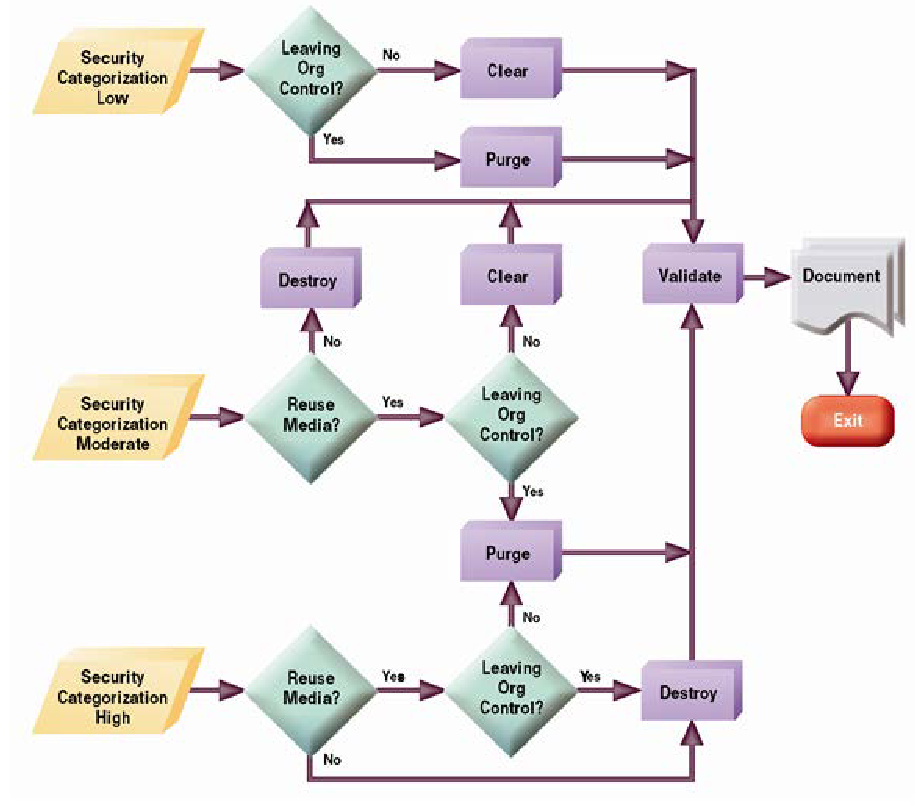
\includegraphics[height=2.5in]{screen1.png}
\caption{CartPole environment}
\label{fig:screen1_chap22}
\end{figure}

In this particular version of the problem, the \emph{action space} is binary, 0 pushes the cart to the left, 1 pushes the cart to the right. Every state is characterized by four \emph{features} $x_1 \ldots x_4$, the cart position ($-4.8 \leq x_1 \leq 4.8$), the cart velocity ($-\infty \leq x_2 \leq \infty$), the pole angle ($-24\degree \leq x_3 \leq 24\degree$), and the pole angular velocity ($-\infty \leq x_4 \infty$). The \emph{rewards} are $+1$ for every step taken. This means the agent has to try to prevent the pole from tipping over to get the greatest return. \emph{Termination} of the episode occurs when the cart is moving out of range (cart position $|x_1| > 2.4$), the pole is tipping over (pole angle $|x_3| > 12\degree$), or the episode length is greater than 200.

The DQN can be implemented using the ''CartPole'' environment\footnote{\url{https://gymnasium.farama.org}. The Farama gymnasium provides a number of reference environments for reinforcement learning.}. First, the required packages are loaded, the environment is created and the number of actions and number of features of a state are determined:

\begin{samepage}
\begin{pythoncode}
import math
import random
import keras
from keras import layers
import gymnasium as gym
import tensorflow as tf
import numpy as np
import pygame

env = gym.make("CartPole-v1", render_mode="human")

Actions = range(0, env.action_space.n)
Ssize = env.observation_space.shape[0]
\end{pythoncode}
\end{samepage}

The next Python code block defines hyperparameters for the neural network and for reinforcement learning:

\begin{samepage}
\begin{pythoncode}
# Neural net parameters
batch_size = 20
dropout = 0.25
activation = 'relu'

# Reinforcement learning parameters
epsilon = 0.05 # epsilon
gamma = 0.9 # discount factor
C = 5*batch_size # When to update weights

# Replay buffer D
D = collections.deque(maxlen=5000)
\end{pythoncode}
\end{samepage}

The functions $\hat{q}_M$ and $\hat{q}_T$ are sequential, fully-connected neural networks with a single output unit, defined in Keras. The output represents the value of $\hat{q}$ computed by the network from its inputs. The inputs are state--action pairs, which is why \\
{\small \texttt{input\_shape=(Ssize+1)}} in the Python code block below which defines the main neural network:

\begin{samepage}
\begin{pythoncode}
# Main network, used to select actions
Q_m = keras.Sequential([
    layers.InputLayer(input_shape=(Ssize+1),
                      batch_size=batch_size,
                      dtype=tf.float32),
    layers.Dense(Ssize*4, activation=activation),
    layers.Dropout(rate=dropout),
    layers.Dense(Ssize*2, activation=activation),
    layers.Dropout(rate=dropout),
    layers.Dense(1, activation='linear')
])
Q_m.compile(loss='huber', optimizer='adam')
\end{pythoncode}
\end{samepage}

Keras provides functions that make cloning a network and getting and setting weights easy. The following Python code block creates the target network as a copy of the main network and sets its weights to those of the main network:

\begin{samepage}
\begin{pythoncode}
# Target network, used to compute targets
Q_t = keras.models.clone_model(Q_m)
Q_t.compile(loss='huber', optimizer='adam')
Q_t.set_weights(Q_m.get_weights())
\end{pythoncode}
\end{samepage}

Getting a value of $\hat{q}$ for some input state-action pair is prediction from the network. The following function prepares the inputs (state features and action) as a Numpy array, adding the minibatch dimension, then selects the first prediction of the first return batch:

\begin{samepage}
\begin{pythoncode}
def getQ(Q, s, a):
    return Q.predict( \
        np.expand_dims(np.array(s.tolist()+[a]), axis=0), \
        verbose=0)[0][0]
\end{pythoncode}
\end{samepage}

The following Python code block implements a convenient max and argmax function over all actions for the $\hat{q}$ values of the main or target network:

\begin{samepage}
\begin{pythoncode}
def maxQ(Q, s, arg):
    maxq = -np.inf
    maxa = None
    for a in Actions:
        q = getQ(Q, s, a)
        if q > maxq:
            maxq = q
            maxa = a
    return maxa if arg else maxq
\end{pythoncode}
\end{samepage}

The policy $\pi$ is an $\epsilon$-greedy policy, defined in Python in the following code block. This uses the main network \texttt{Q\_m}.

\begin{samepage}
\begin{pythoncode}
def pi(s, epsilon):
    if random.random() < epsilon:
        return random.choice(Actions)
    else:
        return maxQ(Q_m, s, True)
\end{pythoncode}
\end{samepage}

The update target for the DQN uses the target network \texttt{Q\_t} and the target expression from Figure~\ref{fig:dqn}. 

\begin{samepage}
\begin{pythoncode}
def target_DQN(Q_t, r, sprime):
    return r + gamma * maxQ(Q_t, sprime, False)
\end{pythoncode}
\end{samepage}

The following function takes a batch of entries of the experience replay buffer and creates training batches of inputs x (state features and action) and target y:

\begin{samepage}
\begin{pythoncode}
def training_xy(batch):
    x = np.zeros((batch_size, Ssize+1))
    y = np.zeros(batch_size)
    for i, (s, a, r, t, sprime) in enumerate(batch):
        x[i] = list(s) + [a]
        if t == 1:
            y[i] = r
        else:
            y[i]=target_DQN(Q_t, r, sprime)
    return x, y
\end{pythoncode}
\end{samepage}

The final block of Python code is the DQN algorithm, a straightforward implementation of Figure~\ref{fig:dqn}\footnote{A complete implementation is available at \url{https://github.com/jevermann/busi4720-rl/blob/main/DDQN_tuples.py}.}. The SGD update step is done using the Keras function \texttt{train\_on\_batch} that trains the network on a single batch of data.

\begin{samepage}
\begin{pythoncode}
t = 0
for episode in range(max_episodes):
    s = env.reset()[0]
    terminal = False
    while not terminal:
        a = pi(s, epsilon)
        sprime, r, terminal, _, _ = env.step(a)
        t += 1
        D.append((s, a, r, int(terminal), sprime))
        s = sprime
        if t >= batch_size:
            batch = random.sample(D, batch_size)
            x, y = training_xy(batch, ddqn=False)
            loss = Q_m.train_on_batch(x=x, y=y)

        if t % C == 0:
            Q_t.set_weights(Q_m.get_weights())
\end{pythoncode}
\end{samepage}

\subsubsection*{Double DQN}

An extension to the DQN algorithm is the Double DQN (DDQN)\index{Double DQN} \index{DDQN|see{Double DQN}}. It is based on the idea of Double-Q learning for tabular methods and uses the the target network $\hat{q}_T$ as a second $Q$ function. This removes the upward bias from using the \emph{max()} function as target estimator. The only change to be made is in the definition of the target, which, for a DDQN is: 

\begin{align*}
& \text{Target}\;y_j \leftarrow \begin{cases} r_j & \qquad \text{if $S_{j+1}$ is terminal} \\
r_j + \gamma \hat{q}_T (S_{j+1}, \operatorname*{argmax}_{A'} \hat{q}_M (S_{j+1}, A') ) & \qquad \text{otherwise}\end{cases} \hspace{1in}
\end{align*}

In Python, this is a also a simple change:

\begin{pythoncode}
def target_DDQN(Q_m, Q_t, a, r, sprime):
    return r + gamma * getQ(Q_t, sprime, maxQ(Q_m, sprime, False))
\end{pythoncode}

\subsubsection*{Prioritized Replay}

Another extension to the basic DQN algorithm is the use of \emph{prioritized replay}\index{Prioritized replay}. In the DQN algorithm above, sampling from the experience replay buffer was done with uniform probability for all elements in the buffer. However, there are some some elements that are more informative than others, that is, more can be learned from them than from others. In particular, these are the elements that have a large absolute TD error, that is, the elements for which $|y_j - \hat{q}_M (S_j, A_j, \theta_M)|$ is large, where $y_j$ is either the DQN or DDQN target. Intuitively, elements that have a small prediction error are not very informative, as not much can be learned from them. When using prioritized experience replay, the TD errors are calculated when experience tuples are added to the replay buffer. Sampling from the buffer takes the priorities into account. 

\subsubsection*{Dueling DQN}

The Dueling DQN is another extension of the basic DQN algorithm\index{Dueling DQN}. It is based on the \emph{advantage function}, which is the difference between the action value function and the state value function\index{Advantage function}:


\begin{align*}
A(s, a) = Q(s, a) - V(s)
\end{align*}

In other words, the advantage function expresses the advantage of taking action $a$ in state $s$ over the average action in state $s$ that is represented by the state value function. The advantage function can be rewritten as follows:
\begin{align*}
Q(s, a) = V(s) + A(s, a)
\end{align*}

This formulation of the advantage function suggests that the action value function can be composed of two functions. In practice, that means the computation of the action value function is done by two different neural networks, the ''\emph{value stream}'' and the ''\emph{advantage stream}''. Both use the same state features $x$ as input. The advantage stream additionally receives the action $a$ as input. In practice, the value stream and advantage stream use one or more common neural network layers, e.g. dense layers, and then separate to end in two different output nodes, one for the value function and one for the advantage function. The two outputs are then added to calculate the action value function $q$ as follows:

\begin{align*}
Q(s, a, \theta, \alpha, \beta) = V(s, \theta, \beta) + \left( A(s, a, \theta, \alpha) - \frac{a}{|\mathcal{A}|} A(s, a', \theta, \alpha) \right)
\end{align*}

Here, $\theta$ are shared neural-network parameters, $\beta$ are parameters only for the ''value-stream'' neural network, and $\alpha$ are parameters only for the ''advantage-stream'' neural network.

\section{Policy Gradient Methods}

Policy gradient methods optimize the policy directly. Unlike value-based methods, which first estimate the action value function and derive a policy based on these estimates, policy gradient methods adjust the policy parameters $\theta$ directly in response to the received reward. This direct approach enables more nuanced strategies and behaviors, particularly in environments with high-dimensional or continuous action spaces.

Policy gradient methods\index{Policy gradient method} rely on optimizing parameterized policies with respect to the expected return by gradient ascent. The policy is typically represented as 

\begin{align*}
\pi(s, a) = \pi(s, a, \theta) = \Pr(A_t = a | S_t = s, \theta_t = \theta)
\end{align*}

which defines the probability of selecting action $a$ in state $s$, parameterized by $\theta$. 

The objective function in policy gradient methods is defined as:

\begin{align*}
J(\theta) = \mathbb{E}_{\tau \sim \pi_\theta} \left[ R(\tau) \right]
\end{align*}

where $\tau$ denotes a trajectory of states and actions, and $R(\tau)$ is the cumulative reward of the trajectory. The expectation is over all trajectories possible under policy $\pi_\theta$.

Policy gradient methods have a number of advantages over value-based methods such as DQN or DDQN:
\begin{itemize}
\item They are particularly effective in environments with continuous, high-dimensional action spaces.
\item Policy gradient methods can converge to a stable policy due to their gradient-based optimization approach.
\item Unlike value-based methods, they can learn stochastic policies with arbitrary probabilities, which are crucial in environments where randomness plays a role in optimal decision making. They are more flexible than $\epsilon$-greedy policies over action values in approaching deterministic policies.
\end{itemize}

On the other hand, policy gradient methods also have disadvantages, such as:
\begin{itemize}
\item The estimates of the gradient can have high variance, leading to inefficient learning and the need for variance reduction techniques.
\item They often require a large number of samples to converge, making them inefficient.
\item The performance of the policy can be heavily dependent on the initial parameter settings.
\end{itemize}

A simple policy gradient method is REINFORCE\index{REINFORCE|see{Policy gradient method}}. The REINFORCE method uses the following parameter update method. The update is proportional to the return $G_t$ and inversely proportional to the action probability $\pi$. 

\begin{align}
\theta_{t+1} = \theta_t + \alpha G_t \frac{\nabla \pi(A_t | S_t, \theta)}{\pi(A_t | S_t, \theta_t)} \label{eq:reinforce}
\end{align}

A complete Monte Carlo based REINFORCE algorithm is shown in Figure~\ref{fig:reinforce}. The basic structure is similar to the tabular MC control introduced in the previous chapter. Complete episodes are generated and the updates are based on the actual return $G$ at each step. There is no bootstrapping of estimates using other estimates. The primary difference to tabular MC is in the update step that uses the REINFORCE update formula Equation~\ref{eq:reinforce}.

\begin{figure}
\small
\begin{tcolorbox}[colback=code]
\vspace{-\baselineskip}
\begin{align*}
& \text{Input: A differentiable policy}\;\pi(a | s, \theta);\;\text{step size}\; \alpha > 0 \\
& \text{Initialize policy parameters}\; \theta \in \mathbbm{R}^d\;\text{arbitrarily} \\
& \text{Loop forever (for each episode):} \\
& \quad \text{Generate an episode}\; S_0, A_0, R_1, \ldots S_{T-1}, A_{T-1}, R_T, \hspace{1in} \\
& \quad \text{Loop for each step of the episode}\;t=0, 1, \ldots, T-1:\\
& \quad \quad G \leftarrow \sum\nolimits_{k=t+1}^T \gamma^{k - t - 1}R_k \\
& \quad \quad \theta \leftarrow \theta + \alpha G \nabla \ln \pi(A_t | S_t, \theta)
\end{align*}
\end{tcolorbox}
\caption[REINFORCE: Monte-Carlso Control]{REINFORCE: Monte-Carlo Control (episodic) (Source: SB)}
\label{fig:reinforce}
\end{figure}

\subsubsection*{REINFORCE with Baseline}

An extension to the basic REINFORCE method is to use ''baselines''\index{Baseline (in reinforcement learning)}, values relative to which the return $G_t$ is evaluated. This reduces the variance of the updates but leaves the expected values unchanged, that is, it is unbiased. Additionally, this has been shown to improve the speed of learning. 

The main idea is to use the following update that includes a ''baseline'' return $b(S_t)$ for state $S_t$:

\begin{align*}
\theta_{t+1} = \theta_t + \alpha(G_t - b(S_t)) \frac{\nabla \pi(A_t | S_t, \theta)}{\pi(A_t | S_t, \theta_t)}
\end{align*}

One can choose $b(S_t) = \hat{v}(S_t)$, that is to use the state value function as baseline. This yields the following update:

\begin{align*}
\theta_{t+1} = \theta_t + \alpha(G_t - \hat{v}(S_t)) \frac{\nabla \pi(A_t | S_t, \theta)}{\pi(A_t | S_t, \theta_t)}
\end{align*}

A complete implementation is shown in Figure~\ref{fig:reinforcebaseline}. Note that the state value function is also a parameterized function, with parameter vector $w$. The update step must not only update the policy parameters $\theta$ but also the value function parameters $w$. The parameters $w$ are updated using an update step analogous to that of the DQN (Equation~\ref{eq:dqnupdate}) but for the state value function, rather than the action value function.

\begin{figure}
\small
\begin{tcolorbox}[colback=code]
\vspace{-\baselineskip}
\begin{align*}
& \text{Input: A policy}\;\pi(a | s, \theta);\;\text{step size}\; \alpha_\theta > 0 \\
& \text{Input: A state-value function}\;\hat{v}(s, w);\;\text{step size}\; \alpha_w > 0 \\
& \text{Initialize parameters}\; \theta \in \mathbbm{R}^d,\; w \in \mathbbm{R}^d\;\text{arbitrarily} \\
& \text{Loop forever (for each episode):} \\
& \quad \text{Generate an episode}\; S_0, A_0, R_1, \ldots S_{T-1}, A_{T-1}, R_T, \hspace{1in} \\
& \quad \text{Loop for each step of the episode}\;t=0, 1, \ldots, T-1:\\
& \quad \quad G \leftarrow \sum\nolimits_{k=t+1}^T \gamma^{k - t - 1}R_k \\
& \quad \quad \delta \leftarrow G - \hat{v}(S_t, w) \\
& \quad \quad w \leftarrow w + \alpha_w \delta \nabla \hat{v}(S_t, w) \\
& \quad \quad \theta \leftarrow \theta + \alpha_\theta G \nabla \ln \pi(A_t | S_t, \theta)
\end{align*}
\end{tcolorbox}
\caption[REINFORCE with Baseline]{REINFORCE with Baseline (Source: SB)}
\label{fig:reinforcebaseline}
\end{figure}

\subsubsection*{Actor-Critic Methods}

The policy gradient methods in Figures~\ref{fig:reinforce} and \ref{fig:reinforcebaseline} are both Monte Carlo methods. Recall that moving from Monte Carlo method to TD methods involved recognizing that $G_{t+1} = R_t + \gamma G_t$ and that the expected values of $G_t$ is the state value of state $S_t$. Starting with the REINFORCE with baseline update function, the same considerations apply to policy gradient methods.

\begin{align*}
\theta_{t+1} &= \theta_t + \alpha (G_{t} - \hat{v}(S_t)) \frac{\nabla \pi(A_t | S_t, \theta)}{\pi(A_t | S_t, \theta_t)} \\
&= \theta_t + \alpha (R_{t+1} + \gamma \hat{v}(S_{t+1}, w) - \hat{v}(S_t, w)) \frac{\nabla \pi(A_t | S_t, \theta)}{\pi(A_t | S_t, \theta_t)} \\
&= \theta_t + \alpha \delta_t \frac{\nabla \pi(A_t | S_t, \theta)}{\pi(A_t | S_t, \theta_t)}
\end{align*}

Here, $\delta_t$ is the TD error. The resulting ''\emph{One-Step Actor-Critic}'' method uses bootstrapping to estimate the state value function, that is, it uses estimated values rather than actual returns. Just like TD, SARSA and Q-learning for tabular methods, actor-critic methods\index{Actor-critic method} can improve on the slow learning of Monte Carlo methods and are also useful for non-episodic, continuous problems. Figure~\ref{fig:actorcritic} shows the complete algorithm for the one-step actor-critic method.

\begin{figure}
\small
\begin{tcolorbox}[colback=code]
\vspace{-\baselineskip}
\vspace{-.5\baselineskip}
\begin{align*}
& \text{Input: A policy}\;\pi(a | s, \theta);\;\text{step size}\; \alpha_\theta > 0 \\
& \text{Input: A state-value function}\;\hat{v}(s, w);\;\text{step size}\; \alpha_w > 0 \hspace{1in} \\
& \text{Initialize parameters}\; \theta \in \mathbbm{R}^d,\; w \in \mathbbm{R}^d\;\text{arbitrarily} \\
& \text{Loop forever (for each episode):} \\
& \quad \text{Initialize}\;S\;\text{(first state of episode)}; I \leftarrow 1 \\
& \quad \text{Loop while}\;S\;\text{not terminal (for each time step):} \\
& \quad \quad \text{Sample}\;A\;\text{from}\; \pi(.|S, \theta) \\
& \quad \quad \text{Take action}\;A,\;\text{observe}\;S', R \\
& \quad \quad \delta \leftarrow R + \gamma \hat{v}(S', w) - \hat{v}(S, w) \\
& \quad \quad w \leftarrow w + \alpha_w \delta \nabla \hat{v}(S_t, w) \\
& \quad \quad \theta \leftarrow \theta + \alpha_\theta G \nabla \ln \pi(A_t | S_t, \theta) \\
& \quad \quad S \leftarrow S'; I \leftarrow \gamma I
\end{align*}
\end{tcolorbox}
\caption[One-Step Actor-Critic algorithm]{One-Step Actor-Critic algorithm (Source: SB)}
\label{fig:actorcritic}
\end{figure}

\section{Additional Information}

\subsubsection*{Stable Baselines}

OpenAI Stable Baselines is a collection of RL algorithm implementations. It provides a set of high-quality, efficient, and easy-to-use Python implementations of several state-of-the-art reinforcement learning algorithms. The primary goal of Stable Baselines is to make it simpler for the research community and industry practitioners to replicate, refine, and deploy RL solutions. Stable Baselines has several features that are designed to enhance the usability and performance of RL algorithms:

\begin{itemize}
    \item \emph{Unified Structure:} Each algorithm adheres to a consistent structure, making it easy to understand, modify, and experiment with different algorithms.
    \item \emph{Pre-configured Hyperparameters:} It comes with expert-selected hyperparameters that work well out of the box for many problems, reducing the need for extensive tuning.
    \item \emph{Extensive Documentation and Examples:} Comprehensive documentation and a variety of examples are provided, facilitating quick learning and implementation.
\end{itemize}

Stable Baselines includes a wide array of RL algorithms, each tailored for different kinds of RL problems. Some of the notable included algorithms are:

\begin{itemize}
    \item \emph{Proximal Policy Optimization (PPO):} A policy gradient method that balances the benefits of on-policy and off-policy learning, offering both robustness and stability in performance across a variety of environments.
    \item \emph{Deep Q-Network (DQN):} An off-policy algorithm that uses a deep neural network to approximate the Q-value function, suitable for discrete action spaces.
    \item \emph{Soft Actor-Critic (SAC):} An actor-critic method that optimizes a stochastic policy and aims for maximizing expected return while also maximizing entropy, making it effective for continuous action spaces.
    \item \emph{A2C and A3C:} Synchronous (A2C) and Asynchronous (A3C) Advantage Actor-Critic methods that use multiple workers to explore the environment and learn more efficiently.
\end{itemize}

\begin{tcolorbox}[colback=code]
\small
\url{https://stable-baselines.readthedocs.io/en/master/}
\normalsize
\end{tcolorbox}

\subsubsection*{Gymnasium}

Farama Gymnasium extends the OpenAI Gym framework, providing a suite of RL environments designed for research and education. The Gymnasium environments range from simple toy problems to complex simulations that mimic real-world scenarios. Farama Gymnasium offers several features that make it a useful resource:

\begin{itemize}
\item \emph{Wide Range of Environments:} Includes classic control tasks, algorithmic tasks, Atari games, and physical simulations.
\item \emph{Standardized APIs:} Maintains consistent APIs across different environments, facilitating easy integration and experimentation with various RL algorithms.
\item \emph{Customization and Extensibility:} Allows for customization of environments and easy addition of new ones, enabling researchers to test algorithms on tailor-made scenarios.
\item \emph{Community-Driven:} Open-source and community-driven, which encourages contributions and continuous improvement.
\end{itemize}

The environments in Farama Gymnasium can be categorized into several types, each suited for specific aspects of reinforcement learning:

\begin{itemize}
\item \emph{Classic Control:} Simple mechanics and dynamics, such as CartPole, MountainCar, and Pendulum, which are excellent for initial algorithm testing and teaching fundamentals.
\item \emph{Atari Games:} Emulated Atari 2600 video games, providing a range of challenges from simple to complex decision-making and control in pixel-based environments.
\item \emph{Algorithmic Tasks:} Environments that require the agent to learn underlying algorithms to perform tasks like sorting numbers and simple arithmetic.
\item \emph{2D and 3D Robots:} Simulations of robotic tasks including walking, picking, and moving objects, which are more complex and require continuous control strategies.
\end{itemize}

\begin{tcolorbox}[colback=code]
\small
\url{https://gymnasium.farama.org/index.html}
\normalsize
\end{tcolorbox}

\subsubsection*{AlphaGo}

AlphaGo\index{AlphaGo} is a significant achievement in the field of artificial intelligence, developed by Google DeepMind. It was designed to play the ancient board game Go, which is known for its deep strategic complexity.  AlphaGo's architecture showcases the potential of deep learning and reinforcement learning techniques. AlphaGo combines advanced machine learning techniques, including deep neural networks and Monte Carlo tree search (MCTS). Its design consists of several key components:

\begin{itemize}
\item \emph{Policy Networks:} These networks were used to predict the next move during a game. AlphaGo was trained on both human expert games and games it played against itself.
\item \emph{Value Networks:} This network predicted the winner of the game from the current position, assisting AlphaGo in evaluating board positions.
\item \emph{Monte Carlo Tree Search:} MCTS was utilized to simulate various possible future game scenarios, guiding the policy and value networks to explore the most promising moves further.
\end{itemize}

\begin{figure}
\begin{center}
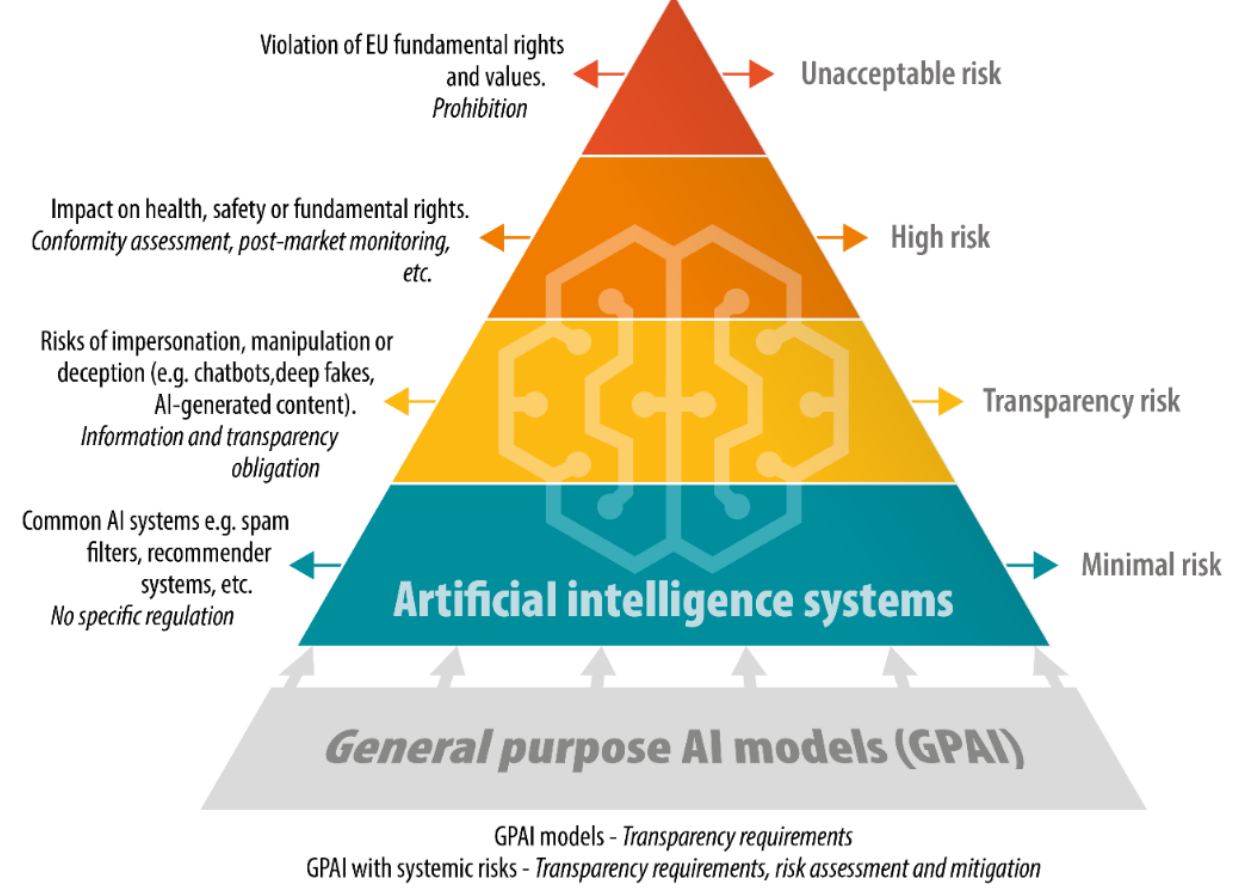
\includegraphics[width=.5\textwidth]{screen2} \\
\footnotesize \url{https://www.alphagomovie.com}
\end{center}
\caption{AlphaGo -- The Documentary}
\label{fig:alphago}
\end{figure}

The award-winning full-length documentary ''AlphaGo'' (Figure~\ref{fig:alphago}) chronicles the journey of the AI program from its initial development through its historic 2016 match against Lee Sedol, one of the world's top Go players. It provides an in-depth look at the human and technical narratives behind AlphaGo's development. The film highlights several key aspects of RL.

\begin{tcolorbox}[colback=code]
\small
\url{https://www.alphagomovie.com} \\

\url{https://www.youtube.com/watch?v=WXuK6gekU1Y}
\normalsize
\end{tcolorbox}

The introductory paper on AlphaGo by David Silver and others in the journal Nature should be easy to understand: ''\href{https://www.nature.com/articles/nature24270}{Mastering the game of Go without human knowledge}''. Nature. 550 (7676): 354--359

\section{Additional Learning Materials}

Many well-known and well-published researchers and many companies are actively providing learning materials that can be used to supplement this chapter. They range from introductory materials to full courses on reinforcement learning and are freely available. These researchers and organizations are at the forefront of RL research and the following materials are immensely helpful in understanding this topic.

\paragraph*{David Silver}
Dr. David Silver of University College London is also a lead researchers with Google DeepMind and contributed extensively to the AlphaGo team. He has an excellent introductory course on reinforcement learning with class materials (from 2015) and lectures in a YouTube playlist. Updated courses (2018, 2021) are available on the DeepMind YouTube channel. The 2021 course include topics on deep reinforcement learning. \\

\begin{tcolorbox}[colback=code]
\footnotesize
\url{https://www.davidsilver.uk/} \\

\url{https://www.davidsilver.uk/teaching/} \\

\url{https://www.youtube.com/playlist?list=PLqYmG7hTraZDM-OYHWgPebj2MfCFzFObQ}. \\

\url{https://www.youtube.com/@Google_DeepMind/playlists}.
\end{tcolorbox}

\paragraph*{UC Berkeley}

UC Berkeley hosted a Deep RL Bootcamp in 2017 with slides and lecture videos available online. Additionally, UC Berkeley's course on Deep RL is available online, with lecture slides and videos of past years.

\begin{tcolorbox}[colback=code]
\footnotesize
\url{https://sites.google.com/view/deep-rl-bootcamp/lectures} \\

\url{https://rail.eecs.berkeley.edu/deeprlcourse/}
\end{tcolorbox}


\paragraph*{Denny Britz}

Formerly at the Google AI team, Denny Britz applied RL algorithms to financial markets and trading. He has a interesting blog, and a GitHub repository with resources and algorithm implementations of popular RL algorithms. \\

\begin{tcolorbox}[colback=code]
\footnotesize
\url{https://dennybritz.com/} \\

\url{https://github.com/dennybritz/reinforcement-learning}
\end{tcolorbox}


\paragraph*{Massimiliano Patacchiola} 

Dr. Patacchiola is a postdoc at Cambridge University. He has written a series of excellent blog posts on reinforcement based on the book ''Artificial Intelligence -- A Modern Approach'' by Russell and Norvig. There are lots of illustrations and pointers to implementation and code in multiple languages. \\

\begin{tcolorbox}[colback=code]
\footnotesize
\url{https://github.com/mpatacchiola/dissecting-reinforcement-learning}
\end{tcolorbox}

\paragraph*{Pascal Poupart}

Dr. Poupart of the University of Waterloo has made available videos and all course materials for all lectures for a course on reinforcement learning at UWaterloo. \\

\begin{tcolorbox}[colback=code]
\footnotesize
\url{https://www.youtube.com/playlist?list=PLdAoL1zKcqTXFJniO3Tqqn6xMBBL07EDc} \\

\url{https://cs.uwaterloo.ca/~ppoupart/teaching/cs885-spring18/schedule.html}
\end{tcolorbox}


\paragraph*{Andrew Ng}

Dr. Ng of Stanford University was the former head of Google Brain and chief scientist at Baidu. He has taught an introductory class on reinforcement learning, as part of a broader course on machine learning. \\

\begin{tcolorbox}[colback=code]
\footnotesize
\url{https://www.andrewng.org/} \\

\url{https://www.youtube.com/watch?v=RtxI449ZjSc} \\

\url{https://www.youtube.com/playlist?list=PLA89DCFA6ADACE599}
\end{tcolorbox}


\paragraph*{Andrej Karpathy}

Andrej Karpathy was a founding member of OpenAI (makers of ChatGPT and Dall-E) and later became the Tesla lead for their Autopilot autonomous driving program. An early blog post by Andrei Karpathy on RL is at the introductory level. \\

\begin{tcolorbox}[colback=code]
\footnotesize
\url{https://karpathy.ai/} \\

\url{https://karpathy.github.io/2016/05/31/rl/}
\end{tcolorbox}


\paragraph*{Lilian Weng}

Dr. Weng is a lead researchers at OpenAI (makers of ChatGPT and Dall-E). She has written an early blog post on RL and another one on policy gradient algorithms. \\

\begin{tcolorbox}[colback=code]
\footnotesize
\url{https://lilianweng.github.io/} \\

\url{https://lilianweng.github.io/posts/2018-02-19-rl-overview/}\\

\url{https://lilianweng.github.io/posts/2018-04-08-policy-gradient/}
\end{tcolorbox}


\paragraph*{OpenAI}

OpenAI (makers of ChatGPT and Dall-E) post regularly on their blog, on all things deep learning and also reinforcement learning. The blog posts are easy introduction to a variety of analytics topics. \\

\begin{tcolorbox}[colback=code]
\footnotesize
\url{https://openai.com/blog/openai-baselines-ppo/} \\

\url{https://openai.com/blog/evolved-policy-gradients/} \\

\url{https://openai.com/blog/evolution-strategies/}
\end{tcolorbox}

\section{Review Questions}

\paragraph*{Introduction}
\begin{enumerate}[nosep]
	\item Explain the concept of function approximation in the context of reinforcement learning. How does it address the scalability issues faced by tabular methods?
    \item How does function approximation help in generalizing from seen to unseen states?
    \item Can decision trees be used as function approximators in RL? Discuss their potential advantages and limitations if used.
    \item Describe how function approximation can be applied to state values, action values, and policies. Provide the mathematical representation used for each.
    \item How does function approximation contribute to the flexibility and efficiency of reinforcement learning models?
    \item Provide an example scenario in reinforcement learning where generalization from seen to unseen states would be crucial.
    \item Discuss the issues of stability and convergence in function approximation methods, especially when combined with off-policy learning.
    \item What measures can be taken to prevent overfitting in function approximation models, particularly those using deep neural networks?
    \item Given the advantages and challenges of function approximation, in what types of reinforcement learning problems would you recommend its use?
    \item Imagine you are designing a function approximation model for an RL problem in a financial trading environment. What factors would you consider in choosing the type of function approximator? 
 \end{enumerate}

\paragraph*{Value-Based Methods and Stochastic Gradient Descent}

\begin{enumerate}[nosep,resume*]
	\item What is the formula for the value error (VE) in the context of action values and how is it computed?
    \item Derive the gradient of the MSE loss function used in the context of function approximation for reinforcement learning.
	\item Describe the parameter update rule in stochastic gradient methods for function approximation. What does each term in the update equation represent?
    \item What is bootstrapping in the context of reinforcement learning? How is it implemented in SGD updates?
    \item Describe the concept of experience replay and its significance in stabilizing the SGD updates in reinforcement learning.
    \item Discuss the role of the target network in the Double Q Network (DQN) algorithm. How does it contribute to the stability of the learning process?
    \item Compare the update steps in tabular SARSA and semi-gradient SARSA using function approximation. What is the key difference?
    \item Explain how the stochastic gradient SARSA algorithm is adapted to utilize a replay buffer and target network in the context of the DQN algorithm.
    \item What are the components of the "deadly triad" in reinforcement learning? Describe how each component contributes to instability and divergence.
    \item Provide examples of how modern reinforcement learning algorithms address the challenges posed by the deadly triad.
    \item Explain the impact of periodic updates from the main network to the target network. How does this timing affect the algorithm's performance?
    \item In the context of function approximation, how is the learning process affected when using non-linear function approximators like neural networks compared to linear approximators?
\end{enumerate}

\paragraph*{Policy Gradient Methods}

\begin{enumerate}[nosep,resume*]

	\item Describe how policy gradient methods optimize the policy parameters directly. What is the significance of this approach in environments with continuous action spaces?
    \item Explain the typical representation of a policy in policy gradient methods and how it relates to the probability of selecting actions.
    \item Define the objective function $J(\theta)$ used in policy gradient methods. What does this function represent?
    \item List and describe the main advantages of using policy gradient methods over value-based methods in reinforcement learning.
    \item Explain the principle behind the REINFORCE algorithm. How does it update the policy parameters?
    \item Describe the update rule of the REINFORCE method. How does the inclusion of the logarithm of the policy's probability function influence the update?
    \item Explain why the REINFORCE algorithm updates parameters only at the end of each episode. What are the limitations of this approach?
    \item What is the purpose of using a baseline in the REINFORCE algorithm? How does it affect the variance of the updates?
    \item Explain the update formula used in REINFORCE with baseline. How does the inclusion of the baseline value $b(S_t)$ change the update mechanism?
    \item Compare the REINFORCE algorithm to Actor-Critic methods. How do Actor-Critic methods improve upon the basic policy gradient approach?
    \item How does the One-Step Actor-Critic algorithm use the current and next state values to update the policy and value function parameters?
    \item Explain how the Actor-Critic method combines the benefits of policy gradient and value function approximation methods. What are the specific roles of the "actor" and the "critic"?
\end{enumerate}
